\paragraph{Types of entities}
Three types of entities have been identified
\begin{itemize}
  \item \textit{Active}: entity capable to start an action by itself if provided 
the necessary computational resources;
  \item \textit{Reactive}: entity that only reacts to provided inputs, 
not capable to start an action by itself;
  \item \textit{Passive}: a stateless entity.
\end{itemize}
\begin{table}[H]
\centering
\begin{tabular}{|l|l|}
\hline
\rowcolor{BlueGreen}
Type     & Entities                                 \\ \hline
Active   & pedestrian, bicycle, motorcycle, car, bus, semaphore \\ \hline
Reactive & road, crossroads, sidewalk, bike lane, crossing, house \\ \hline
Passive  & road signs                               \\ \hline
\end{tabular}
\caption{Types of entities}
\label{tab:entity_type}
\end{table}
The entities have the following dependencies:
\begin{itemize}
  \item \textit{Active} provides inputs to \textit{Reactive} (solid line);
  \item \textit{Active} and \textit{Reactive} can use \textit{Passive}, the dependency is not strict (dashed line).
\end{itemize}
\begin{figure}[H]
  \centering
  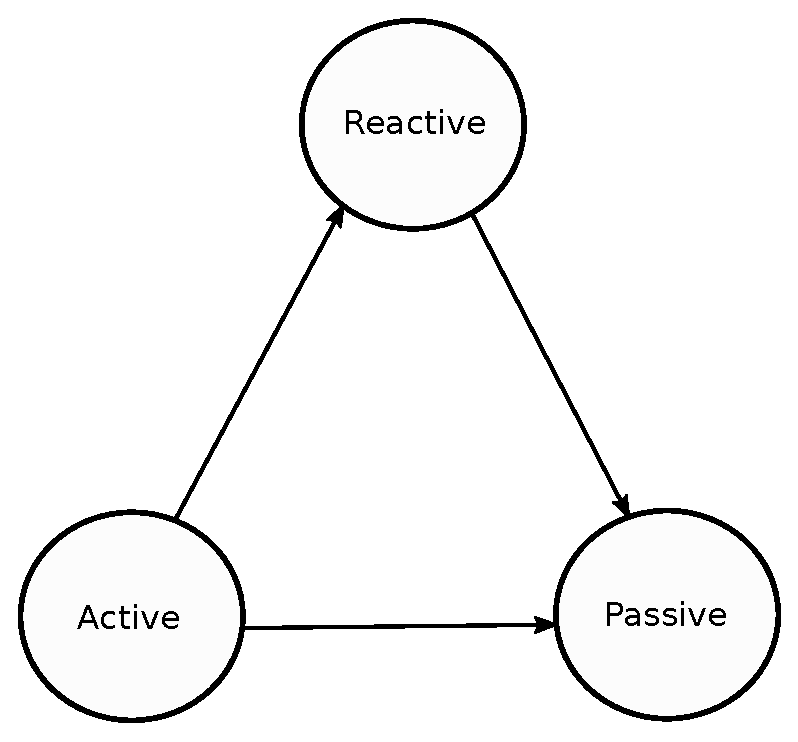
\includegraphics[width=.35\columnwidth]{sections/images/solution/entity_type_dependency.eps}
  \caption{Dependencies between entity types}
  \label{fig:sd-entity-types-deps}
\end{figure}
